\section{Task 2: The symbol sheets and the retraining of the classifier}
\sectionmark{Task 2: Symbol sheets and retraining}
\label{sec:t2}

\subsection{Purpose, conditions and criterion}

\begin{plain}{Task 2 at a glance}
\textbf{Purpose.} The classifier of the quick start has learned from synthetic drawings only: it
has never seen a photograph taken by the board. In this task every symbol is photographed
through the real lens. The 18 blocks of the symbol sheets are photographed three times each,
the 54 photographs are cut into 1{,}890 labelled images of single symbols (\term{crops}), and
the network is trained again on the synthetic and the real images together. Crops from
photographs that the training never sees then measure the accuracy of the classifier on real
symbols, for which the project's target is 95\,\%.

\textbf{Before you begin.} Task~1 is complete: the stand is at its sheet position, the
orientation is settled, and the nine printed sheet pages are at hand. The quick start of the
Set-up Guide has been completed on this laptop with the neural network, so that the synthetic
training set and the file \file{models\bs symbols\_v1.keras} exist. The laptop is connected
to its charger.

\textbf{Complete when.} (1)~All 54 photographs have been cropped, none was skipped, and every
debug picture has been inspected. (2)~The network has been retrained, and its accuracy on the
held-out real crops is recorded. (3)~The retrained classifier reads the simulated test lines
no worse than the old one. (4)~The classifier has been uploaded for the team, and the
photographs are stored in the team's shared folder.

\textbf{Time.} About 45 minutes of photography, 20 minutes of cropping and inspection, about
one hour of unattended training, and 20 minutes of evaluation and upload.
\end{plain}

\subsection{What is being photographed}

\begin{figure}[H]
\centering
\begin{minipage}[c]{0.36\linewidth}\centering
\fbox{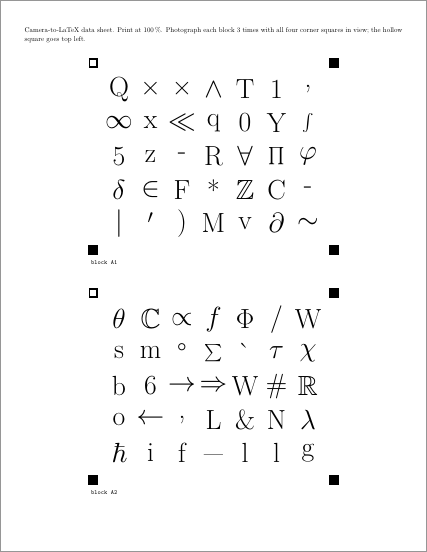
\includegraphics[width=0.95\linewidth]{img/sheet_page.png}}
\end{minipage}\hfill
\begin{minipage}[c]{0.60\linewidth}\centering
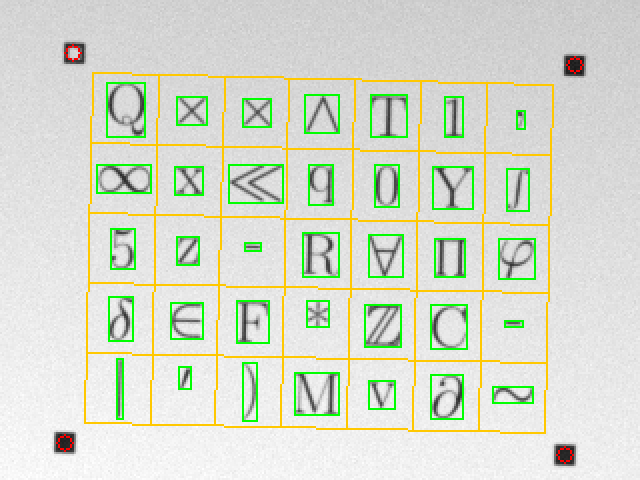
\includegraphics[width=\linewidth]{img/sheet_debug.png}
\end{minipage}
\caption{Left: page~1 of the symbol sheets, with the blocks A1 and A2. Right: a simulated
photograph of block~A1 as the cropping program marks it for inspection: a circle on each corner
square, the grid of cells, and a box around the ink found in each cell.}
\label{fig:sheet}
\end{figure}

Each of the nine pages carries two \term{blocks}. A block is a grid of 35 symbols in five rows
of seven, with a small square at each of its four corners (Figure~\ref{fig:sheet}). Three of the
squares are filled and one, at the top left, is hollow. The cropping program finds the grid by
these squares, and it knows from the file \file{sheets\bs layout.json} which symbol was printed
in which cell, so that every piece of ink it cuts out receives its correct label without
anybody typing it. The name of a block is printed in small type below it. The eighteen blocks
form three sets of six: in the blocks A1 to A6 the letters are upright, as in text; in B1 to B6
they are italic, as in formulas; C1 to C6 mix the two. Together the three sets contain each of
the 182 symbols at least three times, and symbols that are easily confused more often.

Each block is photographed three times, with small changes between the photographs, because the
classifier should learn the symbol and not one particular photograph of it. The photographs of
block~A1 are named \file{A1\_1}, \file{A1\_2} and \file{A1\_3}; the list of all 54 names, in
the order of the printed pages, is the file \file{sheets\bs photo\_names.txt}.

\subsection{Photograph the eighteen blocks}

\step{Prepare the stand}
Remove the line platform, so that pages lie on the desk at the sheet position. Check that the
blank white sheets still cover the desk below the camera and that the lamps stand as in Task~1.
\checkpoint{The desk below the camera is white and evenly lit.}

\step{Open the project in PowerShell}
% The opening sequence, written out in full. Input wherever a task may begin in a new window.
If a PowerShell window whose prompt begins with \texttt{(.venv)} is still open, use it and go
on to the next step. Otherwise open a new window (click \ui{Start}, type \code|powershell|,
click \ui{Windows PowerShell}) and give the two commands of the opening sequence in it.
\begin{ps}[Opening sequence, command 1 of 2]
cd C:\ee105\camera-to-latex
\end{ps}
\begin{ps}[Opening sequence, command 2 of 2]
.\.venv\Scripts\Activate.ps1
\end{ps}
\checkpoint{The prompt reads:}
\venvprompt


\step{Start the series}\label{st:sheetseries}
\begin{ps}
python -m pipeline.capture --series data\sheets --names-file sheets\photo_names.txt
\end{ps}
The viewfinder of Task~1 opens. Its yellow line reads \emph{1/54\ \ next: A1\_1}: the first of
54 photographs will be saved as \file{A1\_1.png}.
\checkpoint{The viewfinder shows the live picture and the name \emph{A1\_1}.}

\step{Photograph one block three times}\label{st:oneblock}
For each block, in the order in which the viewfinder asks for them:
\begin{enumerate}
\item Lay the page on the desk, its top towards the arrow, with the block named in the
  viewfinder in the middle of the picture. Cover the other block of the page with a blank sheet
  whose edge runs through the middle of the white gap between the two blocks.
\item Check four things in the viewfinder: all four corner squares are inside the picture;
  white paper is visible between each square and the border of the picture; the hollow square
  is at the top left; and no shadow or bright spot lies on the block.
\item Wait until the picture has stood still for two seconds, and press \key{Space}. PowerShell
  prints \emph{saved A1\_1.png}, and the viewfinder asks for \emph{A1\_2}.
\item Push the page about half a centimetre to one side and turn it very slightly, so that its
  edge is no longer exactly parallel to the border of the picture. Check the four things again,
  wait, and press \key{Space}.
\item Push the page half a centimetre the other way, and change the light a little: move one
  lamp by a hand's width, or shade it partly with a sheet of paper. Check, wait, and press
  \key{Space}.
\end{enumerate}
Then go on to the next block. The lower block of a page follows its upper block; move the blank
sheet onto the block that has just been photographed.
\checkpoint{After the 54th photograph the viewfinder closes by itself.}

\begin{note}[Mistakes and interruptions]
If you pressed \key{Space} too early, press \key{B}: the viewfinder goes back one name, and the
next \key{Space} replaces the faulty photograph. The series may be interrupted at any time with
\key{Q}. When the command of Step~\ref{st:sheetseries} is given again, it begins once more at
\emph{A1\_1}; names that already have a photograph are marked \emph{(exists)}, and \key{N}
passes over them one at a time without saving.
\end{note}

\begin{caution}[The page must not be turned]
A page that is photographed upside down is recognized only if the hole of its hollow square is
visible in the photograph, and at this distance the hole is only a few pixels wide. If
the hole cannot be made out, the program takes the page to be upright; a page that was in fact
turned would then give every one of its 35 crops the label of another symbol, and the
classifier would be trained on false examples. Always lay the page with its top towards the
arrow.
\end{caution}

\step{Count the photographs}
\begin{ps}
(Get-ChildItem data\sheets -Filter *.png).Count
\end{ps}
\checkpoint{The answer is \texttt{54}.}

\subsection{Cut the photographs into crops}

\step{Run the cropping program}\label{st:crop}
\begin{ps}
python -m tools.crop_sheet --debug
\end{ps}
For each photograph the program finds the four corner squares, lays the grid over the block,
assigns each piece of ink to the cell in which its centre lies, and saves one crop per cell,
cut and scaled exactly as the pipeline later cuts the symbols of a line. It takes a few
seconds.
\begin{out}[What you should see (shortened; the number of pixels will differ)]
A1_1.png: 35 crops, capitals 20 px
A1_2.png: 35 crops, capitals 20 px
A1_3.png: 35 crops, capitals 21 px
...
C6_3.png: 35 crops, capitals 20 px

1890 crops from 54 photos -> C:\ee105\camera-to-latex\data\crops_real
\end{out}
\checkpoint{The last line reports crops from 54 photographs, and no line contains the word
\emph{skipped}.}

The lines may carry three kinds of remark, which Table~\ref{tab:cropnotes} explains.

\begin{table}[H]
\centering
\begin{tabular}{L{3.6cm}L{7.6cm}}
\toprule
\multicolumn{1}{c}{\hd{Remark}} & \multicolumn{1}{c}{\hd{Meaning and action}} \\
\midrule
\emph{skipped}, with a reason & The four corner squares were not found, or did not form the
  rectangle of a block. The photograph yields no crops. Take it again (Step~\ref{st:retake}). \\
\emph{empty cells}, with names & No ink was found in these cells; usually a very small symbol,
  such as a period, was too faint. One or two such cells in a photograph are acceptable. With
  three or more, take the photograph again in better light. \\
\emph{read as an upright page} & The hole of the hollow square was not visible, and the page was
  taken to be upright. This is harmless if the page lay with its top towards the arrow; the
  inspection of the next step confirms it. \\
\bottomrule
\end{tabular}
\caption{Remarks of the cropping program.}
\label{tab:cropnotes}
\end{table}

\step{Inspect the debug pictures}\label{st:debug}
\begin{ps}
explorer data\sheets\debug
\end{ps}
The folder contains one picture for each photograph, in which the program has drawn what it
found (Figure~\ref{fig:sheet}, right). In the Explorer window choose
\menu{View}\then\menu{Extra large icons} and look at all 54 pictures. Each must satisfy three
conditions.
\begin{enumerate}
\item The symbols stand upright, and the square at the top left of the block is the hollow one.
\item The orange grid lines run through the white space between the symbols and do not cut
  through any symbol.
\item Every cell contains exactly one green box, and the box encloses the whole symbol,
  including the dot of an \emph{i} and both parts of an equals sign.
\end{enumerate}
\checkpoint{All 54 pictures satisfy the three conditions. Note the names of any that do not;
they are taken again in the next step.}

\step{Take faulty photographs again}\label{st:retake}
This step is needed only if a photograph was skipped, had three or more empty cells, or failed
the inspection. Give the capture command with the names of those photographs, separated by
commas and without spaces, in place of the yellow placeholder:
\begin{center}
\mbox{\footnotesize\texttt{python -m pipeline.capture -{}-series data\textbackslash{}sheets -{}-names "}\ph{NAMES}\texttt{"}}
\end{center}
\begin{out}[Example only: the command for retaking A3\_2 and B1\_1]
python -m pipeline.capture --series data\sheets --names "A3_2,B1_1"
\end{out}
The quotation marks are necessary: without them PowerShell splits the list at the commas. Then
repeat Steps~\ref{st:crop} and~\ref{st:debug}; the new crops replace the old ones.
\checkpoint{The cropping program reports 54 photographs and no longer names the retaken ones
as faulty.}

\step{Look at the crops themselves}
\begin{ps}
explorer data\crops_real
\end{ps}
The folder contains one subfolder for each of the 159 classes of the classifier. A class is
either a single symbol, such as \file{upper\_A} or \file{alpha}, or a group of symbols that
cannot be told apart by shape alone and are separated later by their size and position, such as
\file{o0} (the letters o and O, the digit 0 and the degree sign) or \file{lI} (the letter l,
the capital I and the vertical bar). Open five folders of your choice, among them
\file{lower\_g}, \file{alpha} and \file{dot}, with the view set to \menu{Large icons}.
\checkpoint{In each folder all images show the symbol, or the group of symbols, after which the
folder is named: black on white, upright and complete. A folder that contains images of
unrelated symbols betrays a turned page; the name of the photograph is part of each file name,
between the two double underscores.}

\subsection{Retrain the classifier}

\step{Keep the old classifier under another name}
\begin{ps}
Copy-Item models\symbols_v1.keras models\symbols_v0.keras
\end{ps}
\begin{ps}
Copy-Item models\symbols_v1.json models\symbols_v0.json
\end{ps}
From now on \emph{symbols\_v0} is the classifier trained on synthetic images alone, and
\emph{symbols\_v1}, which the pipeline uses, will be replaced by the retrained one.
\checkpoint{Neither command printed anything. (\cmd{Copy-Item} is silent when it succeeds.)}

\step{Measure the old classifier on the real crops}\label{st:before}
\begin{ps}
python -m model.evaluate --model symbols_v0
\end{ps}
\begin{out}[Form of the output (the figures are the result of the measurement)]
C:\ee105\camera-to-latex\data\crops_real (held-out photos): 280 crops, accuracy ...%
flagged as uncertain: ...% (accuracy among the rest ...%)
most common confusions:
  ...
worst classes: ...
per-class table: C:\ee105\camera-to-latex\results\crops_symbols_v0.csv
\end{out}
\checkpoint{The first line reports 280 crops (fewer, if some cells were empty). Enter its
accuracy in the record as the value \emph{before retraining}.}

\rationale{One fifth of the photographs, always the same eight (A6\_3, B5\_1, B6\_3, C2\_1,
C2\_3, C3\_1, C3\_2 and C6\_3), is withheld from training, so that the classifier can be judged
on photographs it has never seen. The old classifier has seen no photograph at all, so the same
280 crops serve as a fair measure before and after. They cover 121 of the 159 classes; the
accuracy on the remaining 38, among them the letters e and n and the digit 5, is not measured
by this figure.}

\step{Prepare the laptop and start the training}\label{st:retrain}
Connect the charger and make sure that the laptop will not go to sleep, as described before the
training step of the quick start (Set-up Guide, Section~8). Then run:
\begin{ps}
python -m model.train
\end{ps}
\begin{out}[What you should see at the start]
synthetic C:\ee105\camera-to-latex\data\synthetic\train.npz: 64600 crops
real crops: 1890 (280 held out for testing)
training on 69435 crops, 159 classes, backend keras
model: 149311 weights
Epoch 1/30
\end{out}
The second line confirms that the real crops were found. Each real crop that is not held out
enters the training set five times, because real crops are few and are the only examples that
match the camera exactly: $61{,}385 + 5 \times 1{,}610 = 69{,}435$. An epoch now takes about one
eighth longer than in the quick start, and the whole training 50 to 80 minutes. The figure
\texttt{val\_accuracy} at the end of each epoch is now the accuracy on the held-out real crops.
\checkpoint{The line \emph{real crops: 1890} is present (a slightly smaller number if cells
were empty), and the epochs are being counted.}

\begin{note}[While the training runs]
The camera is not used by the training. Part~A of Task~4, the photography of the 80 test lines,
can be carried out in the meantime in a second PowerShell window; Section~\ref{sec:t4} gives the
complete commands for opening it. Do not close the window in which the training runs.
\end{note}

\step{Read the result of the training}
When the last epoch has finished, the program lists the most frequent mistakes on the held-out
real crops and prints its summary.
\begin{out}[Form of the output at the end (the figures are the result)]
most common mistakes on held-out real crops:
  ...
{
 "name": "symbols_v1",
 "backend": "keras",
 ...
 "data": {
  "synthetic": 61385,
  "real": 1610,
  "real_repeat": 5,
  "external": 0
 },
 "synthetic_val_accuracy": ...,
 "real_val_accuracy": ...
}
\end{out}
\checkpoint{The summary contains \texttt{"real": 1610} (or slightly fewer) and a value of
\texttt{real\_val\_accuracy}. Enter both accuracies in the record.}

\subsection{Judge the new classifier}

\step{Measure the new classifier on the real crops}\label{st:after}
\begin{ps}
python -m model.evaluate
\end{ps}
The output has the form shown in Step~\ref{st:before}; its last line now names the file
\file{crops\_symbols\_v1.csv}.
\checkpoint{Enter the accuracy in the record as the value \emph{after retraining}, together
with the first three lines under \emph{most common confusions}.}

\step{Decide}\label{st:decide2}
Compare the accuracy with the target of 95\,\%.
\begin{itemize}
\item \textbf{95\,\% or more:} the target is met. Continue with the next step.
\item \textbf{Between 85 and 95\,\%:} look at the list of confusions. If most mistakes fall on
  a few pairs of similar shapes, record the pairs and continue; such pairs are a subject of
  Task~3 and of the final report. If the mistakes are scattered over many classes, carry out
  Section~\ref{sec:round2}.
\item \textbf{Below 85\,\%, or lower than before retraining:} labels are probably wrong.
  Repeat the inspection of Step~\ref{st:debug} with particular attention to upright symbols,
  take the faulty photographs again, and repeat the steps from Step~\ref{st:crop} onwards.
\end{itemize}
The measurement is coarse, and the record should say so: with 280 crops, one crop is 0.36
percentage points, and the statistical uncertainty of a value near 95\,\% is about 1.3 points
(Section~\ref{sec:stat} gives the formula). A result of 94\,\% is therefore neither a clear
failure nor a success; it is recorded as measured.

\step{Compare the two classifiers on whole lines}\label{st:regress}
A classifier that names single crops better should also read lines better, and this is checked
before it is shared. If the 20 development lines have already been photographed (Part~A of
Task~4), compare on them, first with the old classifier and then with the new:
\begin{ps}[Old classifier, real photographs of the development lines]
python -m tools.eval_pipeline --split dev --model symbols_v0 --quiet
\end{ps}
\begin{ps}[New classifier, the same photographs]
python -m tools.eval_pipeline --split dev --quiet
\end{ps}
Each command prints a table like that of the quick start, here for 20 lines. If the
photographs do not exist yet, the commands answer \emph{no photos found}; compare then on the
80 simulated photographs instead, and return to this step after Part~A of Task~4:
\begin{pswide}[Old classifier, simulated photographs]
python -m tools.eval_pipeline --images test_set\synthetic --split all --model symbols_v0
\end{pswide}
\begin{ps}[New classifier, simulated photographs]
python -m tools.eval_pipeline --images test_set\synthetic --split all
\end{ps}
\checkpoint{Enter the number of lines read exactly (the percentage in the row \emph{all},
multiplied by the number of lines) for both classifiers in the record. The new classifier
passes if it reads at least as many of the real development lines as the old one, or, where
only simulated photographs are available, no more than four lines fewer of the 80.}

\begin{iffail}[If the new classifier does not pass]
Do not upload it. Restore the old classifier with the two commands below, and report both
tables to the lead.
\end{iffail}
\begin{ps}[Only if the new classifier is to be discarded, command 1 of 2]
Copy-Item models\symbols_v0.keras models\symbols_v1.keras
\end{ps}
\begin{ps}[Only if the new classifier is to be discarded, command 2 of 2]
Copy-Item models\symbols_v0.json models\symbols_v1.json
\end{ps}

\subsection{Share the classifier and keep the photographs}

\step{Upload the classifier}\label{st:publish}
Files in the folder \file{models} are normally kept out of the repository; the option
\code|-f| in the first command includes these two deliberately.
\begin{ps}
git add -f models\symbols_v1.keras models\symbols_v1.json
\end{ps}
\begin{ps}
git commit -m "Classifier retrained on synthetic and real crops"
\end{ps}
\begin{ps}
git push
\end{ps}
\checkpoint{The output of the last command ends with a line that contains \texttt{main ->
main}. Every other member now receives the classifier with \cmd{git pull}, without training.}

\begin{caution}[One person trains]
From this moment the classifier is a file of the repository. If two members train and both
upload, Git cannot combine the two files. Only the member who carries out this task runs
\cmd{python -m model.train} from now on. A member who has trained by mistake discards the
result with the command \cmd{git restore models}.
\end{caution}

\step{Store the photographs in the shared folder}
The photographs are not part of the repository. Pack them into one file,
\begin{ps}
Compress-Archive -Force -Path data\sheets\*.png -DestinationPath data\sheets.zip
\end{ps}
and upload the file \file{sheets.zip}, which is now in the folder
\file{C:\bs ee105\bs camera-to-latex\bs data}, to the team's shared Google Drive folder: open
the folder in the browser, click \menu{New}\then\menu{File upload}, and select the file.
\checkpoint{The file is visible in the shared folder. The photographs are the only part of the
training data that cannot be regenerated by a command.}

\step{Fill in the record}
\begin{table}[H]
\centering
\begin{tabular}{L{7.4cm}C{3.8cm}}
\toprule
\multicolumn{1}{c}{\hd{Quantity}} & \hd{Value} \\
\midrule
Date; photographs taken; photographs retaken & \\
Crops (of 1{,}890); photographs with empty cells & \\
Capital height reported by the cropping program (range) & \hfill px \\
Held-out crops & \\
Accuracy on held-out real crops before retraining (v0) & \hfill \% \\
Accuracy on held-out real crops after retraining (v1) & \hfill \% \\
\texttt{synthetic\_val\_accuracy} after retraining & \\
Duration of the training & \hfill min \\
Three most common confusions after retraining & \\
Development lines read exactly, v0; v1 (of 20) & \\
Simulated lines read exactly, v0; v1 (of 80) & \\
\bottomrule
\end{tabular}
\caption{Record of Task 2.}
\label{tab:t2record}
\end{table}

\subsection{Contingency: a second round of photographs}
\label{sec:round2}

This subsection is carried out only if Step~\ref{st:decide2} calls for it. Three further
photographs of every block double the number of real examples.

\step{Extend the list of names}
\begin{ps}
python -m tools.make_sheets --photos-per-block 6 --no-pdf
\end{ps}
\begin{out}
18 blocks, 630 cells, 108 photos to take -> C:\ee105\camera-to-latex\sheets
\end{out}
The printed sheets remain valid; only the list \file{sheets\bs photo\_names.txt} has grown, to
six names per block.

\step{Photograph, crop and train again}
Repeat Step~\ref{st:sheetseries}. For each block the viewfinder first shows three names marked
\emph{(exists)}: press \key{N} three times, and then photograph the block three times as in
Step~\ref{st:oneblock}, this time with a different position of the lamps than in the first
round. Then repeat the steps from Step~\ref{st:crop} to Step~\ref{st:regress}. The numbers in
the expected outputs change: 108 photographs, 3{,}780 crops, and 22 held-out photographs with
770 crops, so that the accuracies of the two rounds are not measured on the same crops.
\checkpoint{The accuracy after the second round is entered in the record beside the first.}

\step{Share the extended list}
Before the upload of Step~\ref{st:publish}, add the list of names to the same commit:
\begin{ps}
git add sheets\photo_names.txt
\end{ps}

\begin{note}
If the target is still missed, the project's rule applies: a target that is missed is reported
as measured, and never met by weakening the test. Record the value, continue with Task~3, and
name the remaining confusions in the final report.
\end{note}
